% Artigo no padrão ABNT (NBR 6022, 6023, 10520 e 6028) com a classe abnTeX2.
% Compila no Overleaf sem ajustes: envie artigo.tex, referencias.bib e arquitetura.png.
\documentclass[article, 12pt, oneside, a4paper, english, brazil, sumario=tradicional]{abntex2}

\usepackage[T1]{fontenc}
\usepackage[utf8]{inputenc}
\usepackage{times}
\usepackage{graphicx}
\usepackage{microtype}
\usepackage[alf]{abntex2cite}

\titulo{Arquitetura serverless na AWS com infraestrutura como código e entrega contínua: o caso QuizOps}
\tituloestrangeiro{Serverless architecture on AWS with infrastructure as code and continuous delivery: the QuizOps case}
\autor{Luiz Gustavo Gonçalves Brito\thanks{Aluno do curso de Cloud Computing da FIAP, RM 562192. E-mail: luizg1717@gmail.com.}}
\local{São Paulo}
\data{2026}

\makeatletter
\hypersetup{
  pdftitle={\@title},
  pdfauthor={\@author},
  pdfsubject={Global Solution - Multicloud},
  colorlinks=true, linkcolor=black, citecolor=black, urlcolor=black
}
\makeatother

% Quadro (NBR 14724): tabela de texto, com bordas fechadas.
\newcommand{\quadroname}{Quadro}
\newfloat{quadro}{loq}{\quadroname}

\setlength{\parindent}{1.25cm}
\setlength{\parskip}{0.2cm}
\OnehalfSpacing

\begin{document}
\selectlanguage{brazil}
\frenchspacing

\maketitle

\begin{resumoumacoluna}
Este artigo descreve o projeto e a implementação do QuizOps, uma aplicação web de quiz com ranking e mural de fotos, construída sobre serviços gerenciados da Amazon Web Services (AWS). O objetivo foi obter uma aplicação completa, com autenticação, armazenamento de arquivos e entrega automatizada, sem servidores para administrar e com custo proporcional ao uso. A infraestrutura foi descrita em Terraform, organizada em três camadas (front-end, back-end e dados), e o código é publicado por pipelines do GitHub Actions. O front-end em React é servido pelo Amazon CloudFront a partir de um bucket privado do Amazon S3; a autenticação usa o Amazon Cognito com o protocolo SRP; um API Gateway HTTP valida o token JWT antes de invocar uma única função AWS Lambda, que persiste os dados no Amazon DynamoDB e emite URLs pré-assinadas para o envio direto de fotos ao S3. Os resultados mostram que a solução atende aos requisitos funcionais, pode ser recriada em outra conta com poucos comandos e removida por completo com um único comando. São discutidas as decisões de segurança e custo, as limitações encontradas e a correspondência dos serviços com o Google Cloud, o que indica a portabilidade da arquitetura em um contexto multicloud.

\textbf{Palavras-chave}: computação em nuvem; serverless; infraestrutura como código; Terraform; AWS.
\end{resumoumacoluna}

\renewcommand{\resumoname}{Abstract}
\begin{resumoumacoluna}
\begin{otherlanguage*}{english}
This paper describes the design and implementation of QuizOps, a quiz web application with a leaderboard and a photo wall, built on Amazon Web Services (AWS) managed services. The goal was a complete application, with authentication, file storage and automated delivery, without servers to manage and with costs proportional to usage. The infrastructure was written in Terraform, organized into three layers (front-end, back-end and data), and the code is published by GitHub Actions pipelines. The React front-end is served by Amazon CloudFront from a private Amazon S3 bucket; authentication uses Amazon Cognito with the SRP protocol; an HTTP API Gateway validates the JWT before invoking a single AWS Lambda function, which stores data in Amazon DynamoDB and issues presigned URLs for direct photo uploads to S3. The results show that the solution meets the functional requirements, can be recreated in another account with a few commands and fully removed with a single command. Security and cost decisions, limitations and the mapping of services to Google Cloud are discussed, indicating the portability of the architecture in a multicloud context.

\textbf{Keywords}: cloud computing; serverless; infrastructure as code; Terraform; AWS.
\end{otherlanguage*}
\end{resumoumacoluna}

\textual

\section{Introdução}

A computação em nuvem oferece recursos de computação sob demanda, por autoatendimento e com cobrança medida pelo uso \cite{mell2011}. Dentro desse modelo, a computação serverless leva a abstração adiante: o desenvolvedor publica funções e consome serviços gerenciados, enquanto o provedor cuida da escala, da disponibilidade e da capacidade ociosa \cite{baldini2017,jonas2019}.

O problema tratado neste trabalho é a construção de uma aplicação de quiz para encontros de estudo: cada encontro tem um questionário, os participantes enviam uma foto sobre o tema e disputam um ranking. Os requisitos não funcionais eram custo próximo de zero em períodos sem uso, nenhum servidor para administrar e a possibilidade de outra pessoa recriar o ambiente a partir do repositório.

O objetivo geral é apresentar a arquitetura, as decisões técnicas e a implementação do QuizOps na AWS. Os objetivos específicos são: (a) descrever as camadas da solução e o papel de cada serviço; (b) mostrar como a infraestrutura como código e a entrega contínua tornam o ambiente reproduzível; e (c) discutir segurança, custo, limitações e portabilidade para outro provedor.

O artigo está organizado da seguinte forma: a Seção~\ref{sec:referencial} apresenta o referencial teórico; a Seção~\ref{sec:metodo}, a metodologia; a Seção~\ref{sec:arquitetura}, a arquitetura e a implementação; a Seção~\ref{sec:resultados}, os resultados e a discussão; e a Seção~\ref{sec:conclusao}, as considerações finais.

\section{Referencial teórico}\label{sec:referencial}

\subsection{Computação serverless}

\citeonline{baldini2017} definem serverless como um modelo em que o código roda em resposta a eventos, sem que o desenvolvedor provisione ou gerencie servidores, e em que a cobrança considera apenas o tempo de execução. \citeonline{jonas2019} acrescentam que o modelo combina funções como serviço com serviços de back-end gerenciados, como bancos de dados e armazenamento de objetos, e apontam como vantagens a escala automática e o pagamento por uso.

Na AWS, o serviço de funções é o AWS Lambda, que executa o código em resposta a eventos e escala conforme a demanda \cite{awslambda}. O guia de boas práticas da AWS para aplicações serverless recomenda permissões mínimas por função, serviços gerenciados para estado e observabilidade desde o início \cite{awsserverlesslens}.

\subsection{Infraestrutura como código}

Infraestrutura como código (IaC) é a prática de definir a infraestrutura em arquivos versionados, aplicando a ela as mesmas técnicas usadas no desenvolvimento de software, como revisão, testes e controle de versão \cite{fowler2016}. O Terraform é uma ferramenta de IaC declarativa: o usuário descreve o estado desejado e a ferramenta calcula e executa as mudanças necessárias, por meio de provedores para diferentes plataformas \cite{terraform}. A existência de provedores para vários fornecedores de nuvem, como AWS e Google Cloud \cite{terraformgoogle}, torna a ferramenta adequada a cenários multicloud.

\subsection{Integração e entrega contínuas}

A entrega contínua automatiza o caminho entre uma mudança no repositório e sua publicação. O GitHub Actions executa fluxos de trabalho definidos em arquivos YAML, disparados por eventos do repositório, como um \textit{push} \cite{ghactions}.

\subsection{Autenticação baseada em tokens}

O JSON Web Token (JWT) é um formato compacto para transmitir declarações assinadas entre duas partes \cite{rfc7519}. O protocolo Secure Remote Password (SRP) permite que um cliente prove o conhecimento de uma senha sem enviá-la ao servidor, que armazena apenas um verificador derivado dela \cite{wu1998}. O Amazon Cognito implementa o SRP no fluxo de login e emite tokens JWT ao final da autenticação \cite{awscognitosrp}.

\section{Metodologia}\label{sec:metodo}

Trata-se de uma pesquisa aplicada, conduzida como estudo de caso de desenvolvimento. O trabalho seguiu quatro etapas:

\begin{alineas}
  \item levantamento de requisitos em um documento de produto, com o fluxo de cadastro, quiz, mural e ranking;
  \item registro das decisões técnicas em documentos curtos por tema (autenticação, mural, Lambda, API, dados, front-end, IaC e CI/CD), cada um com referência à documentação oficial;
  \item implementação incremental por camada, primeiro em ambiente local (DynamoDB local e emulador de S3 em contêineres) e depois na AWS, com Terraform;
  \item validação ponta a ponta na nuvem: cadastro, resposta ao quiz, envio de foto e consulta ao ranking.
\end{alineas}

As ferramentas utilizadas foram React 19 com Vite e Tailwind CSS no front-end, Node.js 24 no back-end, Terraform com o provedor AWS para a infraestrutura e GitHub Actions para a entrega. O código-fonte, a documentação e o passo a passo de reprodução estão disponíveis no repositório do projeto \cite{repositorio}, e a demonstração em vídeo está nas referências \cite{video}.

\section{Arquitetura e implementação}\label{sec:arquitetura}

A Figura~\ref{fig:arquitetura} mostra a arquitetura, dividida em três camadas dentro da região \textit{us-east-1}. Todos os recursos seguem o padrão de nome \texttt{recurso-projeto-ambiente}, por exemplo \texttt{lambda-quiz-lab}, e recebem etiquetas padrão definidas no provedor do Terraform.

\begin{figure}[htb]
  \caption{\label{fig:arquitetura}Arquitetura do QuizOps na AWS}
  \begin{center}
    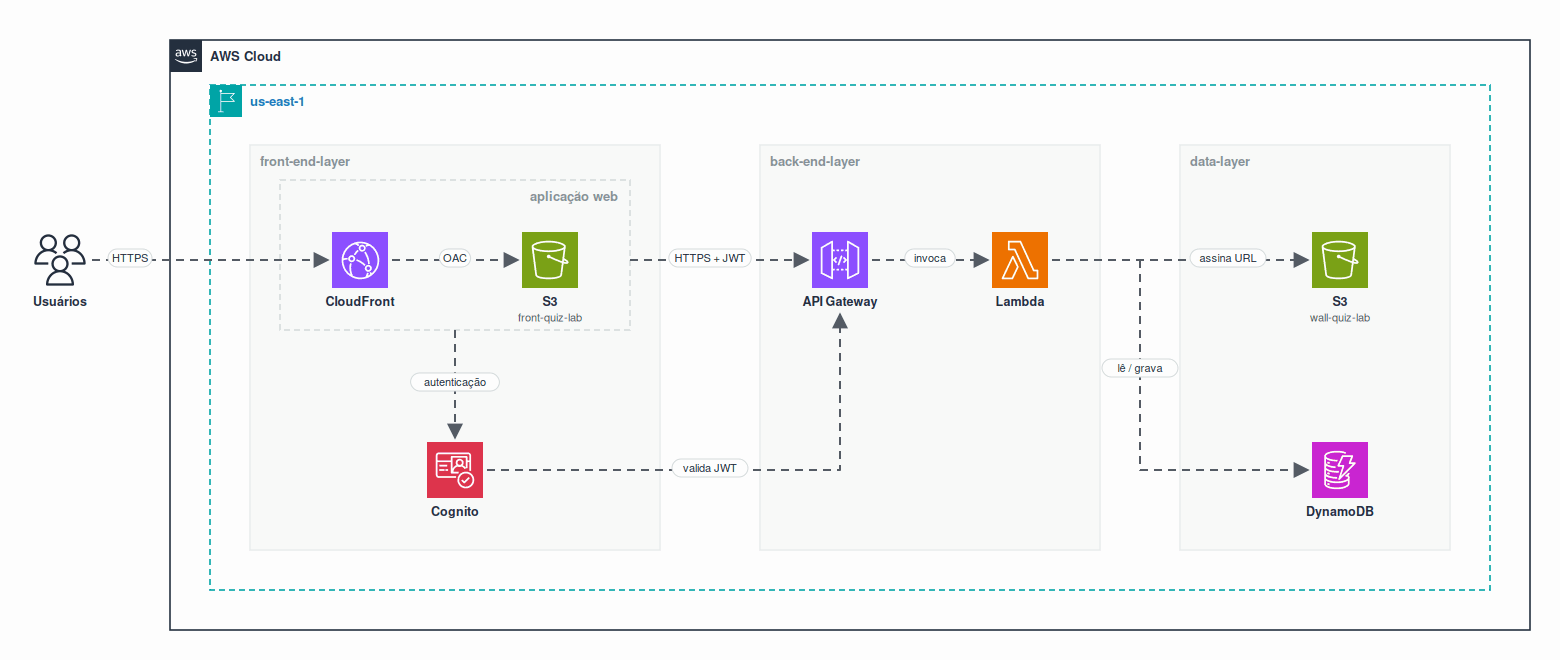
\includegraphics[width=\textwidth]{arquitetura.png}
  \end{center}
  \legend{Fonte: elaborado pelo autor (2026).}
\end{figure}

\subsection{Camada de front-end}

A aplicação React é compilada em arquivos estáticos e publicada em um bucket S3 privado. O Amazon CloudFront distribui esses arquivos por HTTPS no domínio padrão \texttt{*.cloudfront.net}. O acesso ao bucket usa o \textit{Origin Access Control} (OAC): o CloudFront assina as requisições ao S3 e a política do bucket libera a leitura apenas para essa distribuição \cite{awsoac}. Como a aplicação é de página única, o erro 403 do S3 para rotas inexistentes é convertido em \texttt{index.html} com código 200.

O cadastro e o login usam um \textit{user pool} do Amazon Cognito com um \textit{app client} público, sem segredo, já que o código roda no navegador. O login segue o fluxo SRP, de modo que a senha não trafega na autenticação \cite{wu1998,awscognitosrp}.

\subsection{Camada de back-end}

Um API Gateway do tipo HTTP API expõe seis rotas. Um autorizador JWT, configurado com o emissor e a audiência do Cognito, valida o token de cada requisição: token ausente ou inválido recebe a resposta 401 sem que a função seja executada \cite{awsjwt}. Todas as rotas usam uma única integração com uma função Lambda em Node.js 24, que identifica a rota pela combinação de método e caminho e lê o usuário das declarações do token.

A função recebe uma \textit{role} do IAM com permissão para gravar logs e acessar apenas a tabela e o bucket do mural, seguindo o princípio do menor privilégio \cite{awsiam}. O grupo de logs no CloudWatch é criado pelo Terraform antes da função, com retenção de sete dias, para que também seja removido quando o ambiente é destruído.

\subsection{Camada de dados}

As respostas ficam em uma tabela do Amazon DynamoDB em modo sob demanda, cobrada por requisição \cite{awsondemand}. A chave primária combina \texttt{quizId} (partição) e \texttt{userId} (ordenação) \cite{awsdynamo}, o que garante uma resposta por usuário em cada quiz; uma gravação condicional impede uma segunda tentativa. Os questionários ficam em arquivos JSON versionados junto ao código.

As fotos do mural ficam em um bucket S3 privado. O navegador não envia o arquivo à função: ele pede à Lambda uma URL pré-assinada, válida por cinco minutos, e envia a foto diretamente ao S3 \cite{awspresigned}. A mesma técnica, com URLs de leitura, é usada para exibir as fotos. Assim, o tamanho do arquivo não esbarra no limite de carga das invocações síncronas da Lambda \cite{awslambdaquotas} e a função só é cobrada pelo tempo de assinar a URL.

\subsection{Infraestrutura como código e entrega contínua}

A infraestrutura fica em uma única pasta, com um arquivo por serviço, numerados na ordem de dependência, sem módulos. Duas variáveis locais, projeto e ambiente, compõem o nome de todos os recursos; alterá-las permite recriar o ambiente em outra conta sem conflito de nomes de bucket, que são únicos globalmente.

Dois fluxos do GitHub Actions publicam o código a cada \textit{push} na branch principal, cada um disparado apenas por mudanças na sua pasta. O fluxo do front-end compila a aplicação, sincroniza os arquivos com o bucket e invalida o cache do CloudFront; o do back-end empacota o código com as dependências e atualiza a função. A infraestrutura permanece sob responsabilidade do Terraform, fora dos fluxos. O Quadro~\ref{qua:decisoes} resume as principais decisões.

\begin{quadro}[htb]
  \caption{\label{qua:decisoes}Principais decisões técnicas}
  \begin{tabular}{|>{\raggedright\arraybackslash}p{4.2cm}|>{\raggedright\arraybackslash}p{10.5cm}|}
    \hline
    \textbf{Decisão} & \textbf{Justificativa} \\ \hline
    Uma única função Lambda & Menos recursos para gerenciar; rotas resolvidas no código, todas com a mesma permissão. \\ \hline
    HTTP API com autorizador JWT & Requisições não autenticadas são rejeitadas antes de gerar custo de execução. \\ \hline
    URL pré-assinada para fotos & O arquivo não passa pela função, evitando o limite de carga e o custo de transferência. \\ \hline
    DynamoDB sob demanda & Sem capacidade provisionada; custo zero sem requisições. \\ \hline
    Buckets privados e OAC & Nenhum objeto é público; o acesso passa pelo CloudFront ou por URL assinada. \\ \hline
    Domínio padrão do CloudFront & Dispensa domínio e certificado próprios, o que simplifica a reprodução. \\ \hline
    Terraform sem módulos & Um arquivo por serviço, leitura linear e destruição completa com um comando. \\ \hline
  \end{tabular}
  \legend{Fonte: elaborado pelo autor (2026).}
\end{quadro}

\section{Resultados e discussão}\label{sec:resultados}

A aplicação foi publicada e validada na AWS com o fluxo completo: cadastro com confirmação por e-mail, login, resposta ao quiz, envio e visualização de fotos e ranking por encontro e geral. Os dois fluxos de entrega executaram com sucesso, e uma alteração no front-end chega ao CloudFront sem passos manuais.

Quanto à reprodutibilidade, o repositório traz um passo a passo em que outra pessoa faz o \textit{fork}, ajusta o perfil da AWS e o nome do projeto, aplica o Terraform e publica o código pelos fluxos do GitHub Actions, sem instalar dependências da aplicação na própria máquina. O mesmo Terraform remove todos os recursos, inclusive buckets com arquivos e o grupo de logs.

Em segurança, a solução não expõe objetos públicos, não transmite a senha no login, valida o token na borda da API e restringe a função aos recursos que ela usa. Em custo, todos os serviços adotados cobram por uso, o que atende ao requisito de custo próximo de zero sem tráfego.

Foram identificadas as seguintes limitações:

\begin{alineas}
  \item o ranking geral usa uma leitura completa da tabela (\textit{scan}), adequada ao volume de uma turma, mas que deve ser revista com muitos usuários;
  \item os fluxos de entrega usam chaves de acesso estáticas guardadas como segredos do repositório; credenciais temporárias via OpenID Connect são a alternativa recomendada \cite{ghoidc};
  \item o ambiente usa uma única região, sem estratégia de recuperação de desastres.
\end{alineas}

Do ponto de vista multicloud, cada serviço tem um equivalente gerenciado no Google Cloud, como mostra o Quadro~\ref{qua:gcp}. Como o Terraform também possui provedor para o Google Cloud \cite{terraformgoogle}, a mesma abordagem de IaC pode ser aplicada; a migração, porém, exige reescrever os recursos e adaptar o código que usa os SDKs de cada provedor.

\begin{quadro}[htb]
  \caption{\label{qua:gcp}Correspondência entre serviços da AWS e do Google Cloud}
  \begin{tabular}{|>{\raggedright\arraybackslash}p{5cm}|>{\raggedright\arraybackslash}p{9.7cm}|}
    \hline
    \textbf{AWS} & \textbf{Google Cloud} \\ \hline
    Lambda & Cloud Run functions \cite{gcprun} \\ \hline
    API Gateway & API Gateway \cite{gcpapigw} \\ \hline
    Cognito & Identity Platform \cite{gcpidentity} \\ \hline
    DynamoDB & Firestore \cite{gcpfirestore} \\ \hline
    S3 com URL pré-assinada & Cloud Storage com URL assinada \cite{gcpsigned} \\ \hline
    CloudFront & Cloud CDN \cite{gcpcdn} \\ \hline
  \end{tabular}
  \legend{Fonte: elaborado pelo autor (2026).}
\end{quadro}

\section{Considerações finais}\label{sec:conclusao}

O trabalho apresentou o QuizOps, uma aplicação serverless completa na AWS, descrita em Terraform e publicada por entrega contínua. Os objetivos foram atingidos: as camadas e os serviços foram descritos, o ambiente pode ser recriado e removido a partir do repositório, e as decisões de segurança, custo e portabilidade foram discutidas.

Como trabalhos futuros, sugerem-se a troca das chaves estáticas por OpenID Connect nos fluxos de entrega, um índice ou tabela agregada para o ranking geral e a implementação da mesma arquitetura no Google Cloud com Terraform, para comparar custo e esforço entre os provedores.

\bibliography{referencias}

\end{document}
